% =============================================================================
%  kirklin LaTeX  --  neurips-paper template
%  A single-column, NeurIPS-style research paper, built from scratch.
%  Demo content recreates "Attention Is All You Need" (Vaswani et al., 2017)
%  so every moving part is exercised: 8-author block, equal-contribution
%  footnote, the real architecture & attention figures, display equations,
%  three booktabs tables, numbered citations, and an appendix of attention
%  visualizations.
%
%  Figures: the paper's own bundled assets are used —
%    Figures/ModalNet-21.png  (Figure 1, architecture)
%    Figures/ModalNet-19.png  + ModalNet-20.png (Figure 2, attention)
%    vis/*.pdf                (appendix attention visualizations)
%  Prefer a self-contained, image-free build? Swap in figures-tikz-alt.tex,
%  which reproduces Figures 1 and 2 by hand in pure TikZ.
%
%  Build:  latexmk -pdf paper.tex        (handles bibtex passes automatically)
%  Engine: pdflatex (default) — reads the bundled PNG and PDF figures directly.
% =============================================================================
\documentclass[10pt,letterpaper]{article}

% ---- Page geometry: NeurIPS text block is 5.5in wide on US letter ----------
\usepackage[letterpaper,left=1.5in,right=1.5in,top=1in,bottom=1in]{geometry}

% ---- Encoding & fonts (Times text + Times math, the NeurIPS look) ----------
\usepackage[T1]{fontenc}
\usepackage[utf8]{inputenc}
\usepackage{amsmath}
\usepackage{mathtools}
\usepackage{newtxtext}          % Times-like text
\usepackage{newtxmath}          % matching math (provides \mathbb, symbols)
\usepackage{bm}
\usepackage{microtype}          % better justification, fewer overfull boxes

% ---- Graphics, tables, colour ----------------------------------------------
\usepackage{graphicx}           % \includegraphics for the figure assets
\usepackage{booktabs}           % \toprule \midrule \bottomrule
\usepackage{multirow}
\usepackage{array}
\usepackage{xcolor}
\usepackage{caption}

% ---- Section heading style (compact, bold — NeurIPS-ish) -------------------
\usepackage{titlesec}
\titleformat{\section}{\normalfont\large\bfseries}{\thesection}{0.6em}{}
\titleformat{\subsection}{\normalfont\normalsize\bfseries}{\thesubsection}{0.5em}{}
\titleformat{\subsubsection}{\normalfont\normalsize\bfseries}{\thesubsubsection}{0.5em}{}
\titlespacing*{\section}{0pt}{1.6ex plus .2ex}{1.0ex}
\titlespacing*{\subsection}{0pt}{1.2ex plus .2ex}{0.6ex}

\usepackage{enumitem}
\usepackage[numbers,sort&compress]{natbib}   % [1,2] numbered citations
\usepackage{url}

% ---- Hyperlinks (load late) ------------------------------------------------
\definecolor{kirklink}{RGB}{0,90,158}
\usepackage[colorlinks=true,linkcolor=black,citecolor=kirklink,
            urlcolor=kirklink,filecolor=kirklink]{hyperref}

% ---- Caption style: small, bold label --------------------------------------
\captionsetup{font=small,labelfont=bf}

% =============================================================================
%  Reusable macros — math operators & symbols used throughout
% =============================================================================
\DeclareMathOperator{\softmax}{softmax}
\DeclareMathOperator{\Attention}{Attention}
\DeclareMathOperator{\MultiHead}{MultiHead}
\DeclareMathOperator{\Concat}{Concat}
\DeclareMathOperator{\FFN}{FFN}
\DeclareMathOperator{\PE}{PE}
\newcommand{\dmodel}{d_{\mathrm{model}}}
\newcommand{\dff}{d_{\mathrm{ff}}}
\newcommand{\head}{\mathrm{head}}

% ---- Unnumbered footnote (for the equal-contribution note) -----------------
\newcommand\blfootnote[1]{%
  \begingroup
  \renewcommand\thefootnote{}\footnote{#1}%
  \addtocounter{footnote}{-1}%
  \endgroup
}

% =============================================================================
\begin{document}

% ---- Title -----------------------------------------------------------------
\begin{center}
  {\LARGE\bfseries Attention Is All You Need\par}
  \vspace{1.4em}

  % ---- Author grid: 8 authors, 4 per row -----------------------------------
  \newcommand{\authblk}[3]{%
    \begin{tabular}[t]{@{}c@{}}\textbf{#1}\\[1pt] #2\\[1pt]{\small\texttt{#3}}\end{tabular}}
  \authblk{Ashish Vaswani$^{*}$}{Google Brain}{avaswani@google.com}\hspace{1.1em}%
  \authblk{Noam Shazeer$^{*}$}{Google Brain}{noam@google.com}\hspace{1.1em}%
  \authblk{Niki Parmar$^{*}$}{Google Research}{nikip@google.com}\hspace{1.1em}%
  \authblk{Jakob Uszkoreit$^{*}$}{Google Research}{usz@google.com}

  \vspace{1.1em}
  \authblk{Llion Jones$^{*}$}{Google Research}{llion@google.com}\hspace{1.1em}%
  \authblk{Aidan N. Gomez$^{*\dagger}$}{University of Toronto}{aidan@cs.toronto.edu}\hspace{1.1em}%
  \authblk{Łukasz Kaiser$^{*}$}{Google Brain}{lukaszkaiser@google.com}\hspace{1.1em}%
  \authblk{Illia Polosukhin$^{*\ddagger}$}{}{illia.polosukhin@gmail.com}
\end{center}

\blfootnote{$^{*}$Equal contribution. Listing order is random. Jakob proposed
replacing RNNs with self-attention and started the effort to evaluate this idea.
Ashish, with Illia, designed and implemented the first Transformer models and
has been crucially involved in every aspect of this work. Noam proposed
scaled dot-product attention, multi-head attention and the parameter-free
position representation. Niki, Llion, Aidan and Łukasz designed, implemented,
tuned and evaluated countless model variants and the original codebase.\\
$^{\dagger}$Work performed while at Google Brain.\quad
$^{\ddagger}$Work performed while at Google Research.}

% ---- Abstract (centred heading, narrower measure) --------------------------
\begin{center}
\begin{minipage}{0.86\textwidth}
  {\centering\textbf{Abstract}\par}
  \vspace{0.4em}
  \small
  The dominant sequence transduction models are based on complex recurrent or
  convolutional neural networks that include an encoder and a decoder. The best
  performing models also connect the encoder and decoder through an attention
  mechanism. We propose a new simple network architecture, the Transformer,
  based solely on attention mechanisms, dispensing with recurrence and
  convolutions entirely. Experiments on two machine translation tasks show these
  models to be superior in quality while being more parallelizable and requiring
  significantly less time to train. Our model achieves 28.4 BLEU on the WMT 2014
  English-to-German translation task, improving over the existing best results,
  including ensembles, by over 2 BLEU. On the WMT 2014 English-to-French
  translation task, our model establishes a new single-model state-of-the-art
  BLEU score of 41.8 after training for 3.5 days on eight GPUs, a small fraction
  of the training costs of the best models from the literature.
\end{minipage}
\end{center}
\vspace{1em}

% =============================================================================
\section{Introduction}
Recurrent neural networks, long short-term memory~\citep{hochreiter1997long} and
gated recurrent~\citep{cho2014learning} networks in particular, have been firmly
established as state-of-the-art approaches in sequence modeling and transduction
problems such as language modeling and machine translation. Numerous efforts have
since continued to push the boundaries of recurrent language models and
encoder--decoder architectures~\citep{sutskever2014sequence,bahdanau2015neural}.

Recurrent models typically factor computation along the symbol positions of the
input and output sequences. Aligning the positions to steps in computation time,
they generate a sequence of hidden states $h_t$, as a function of the previous
hidden state $h_{t-1}$ and the input for position $t$. This inherently sequential
nature precludes parallelization within training examples, which becomes critical
at longer sequence lengths, as memory constraints limit batching across examples.

Attention mechanisms have become an integral part of compelling sequence modeling
and transduction models, allowing modeling of dependencies without regard to their
distance in the input or output sequences~\citep{bahdanau2015neural,luong2015effective}.
In this work we propose the Transformer, a model architecture eschewing recurrence
and instead relying entirely on an attention mechanism to draw global dependencies
between input and output. The Transformer allows for significantly more
parallelization and can reach a new state of the art in translation quality after
being trained for as little as twelve hours on eight P100 GPUs.

% =============================================================================
\section{Background}
The goal of reducing sequential computation also forms the foundation of the
Extended Neural GPU, ByteNet~\citep{kalchbrenner2016neural} and
ConvS2S~\citep{gehring2017convolutional}, all of which use convolutional neural
networks as basic building block, computing hidden representations in parallel for
all input and output positions. In these models, the number of operations required
to relate signals from two arbitrary input or output positions grows in the
distance between positions, linearly for ConvS2S and logarithmically for ByteNet.
This makes it more difficult to learn dependencies between distant
positions~\citep{hochreiter1997long}. In the Transformer this is reduced to a
constant number of operations, albeit at the cost of reduced effective resolution
due to averaging attention-weighted positions, an effect we counteract with
multi-head attention.

Self-attention, sometimes called intra-attention, is an attention mechanism
relating different positions of a single sequence in order to compute a
representation of the sequence. Self-attention has been used successfully in a
variety of tasks including reading comprehension, abstractive summarization, and
learning task-independent sentence representations~\citep{cheng2016long,
parikh2016decomposable,lin2017structured}. To the best of our knowledge, however,
the Transformer is the first transduction model relying entirely on self-attention
to compute representations of its input and output.

% =============================================================================
\section{Model Architecture}
\label{sec:model}
Most competitive neural sequence transduction models have an encoder--decoder
structure. Here, the encoder maps an input sequence of symbol representations
$(x_1,\dots,x_n)$ to a sequence of continuous representations
$\mathbf{z}=(z_1,\dots,z_n)$. Given $\mathbf{z}$, the decoder then generates an
output sequence $(y_1,\dots,y_m)$ of symbols one element at a time. At each step
the model is auto-regressive, consuming the previously generated symbols as
additional input when generating the next.

The Transformer follows this overall architecture using stacked self-attention and
point-wise, fully connected layers for both the encoder and decoder, shown in the
left and right halves of Figure~\ref{fig:architecture}, respectively.

% ---- FIGURE 1: The Transformer architecture --------------------------------
% Uses the paper's own diagram. Want a dependency-free hand-drawn version
% instead? See figures-tikz-alt.tex.
\begin{figure}[t]
  \centering
  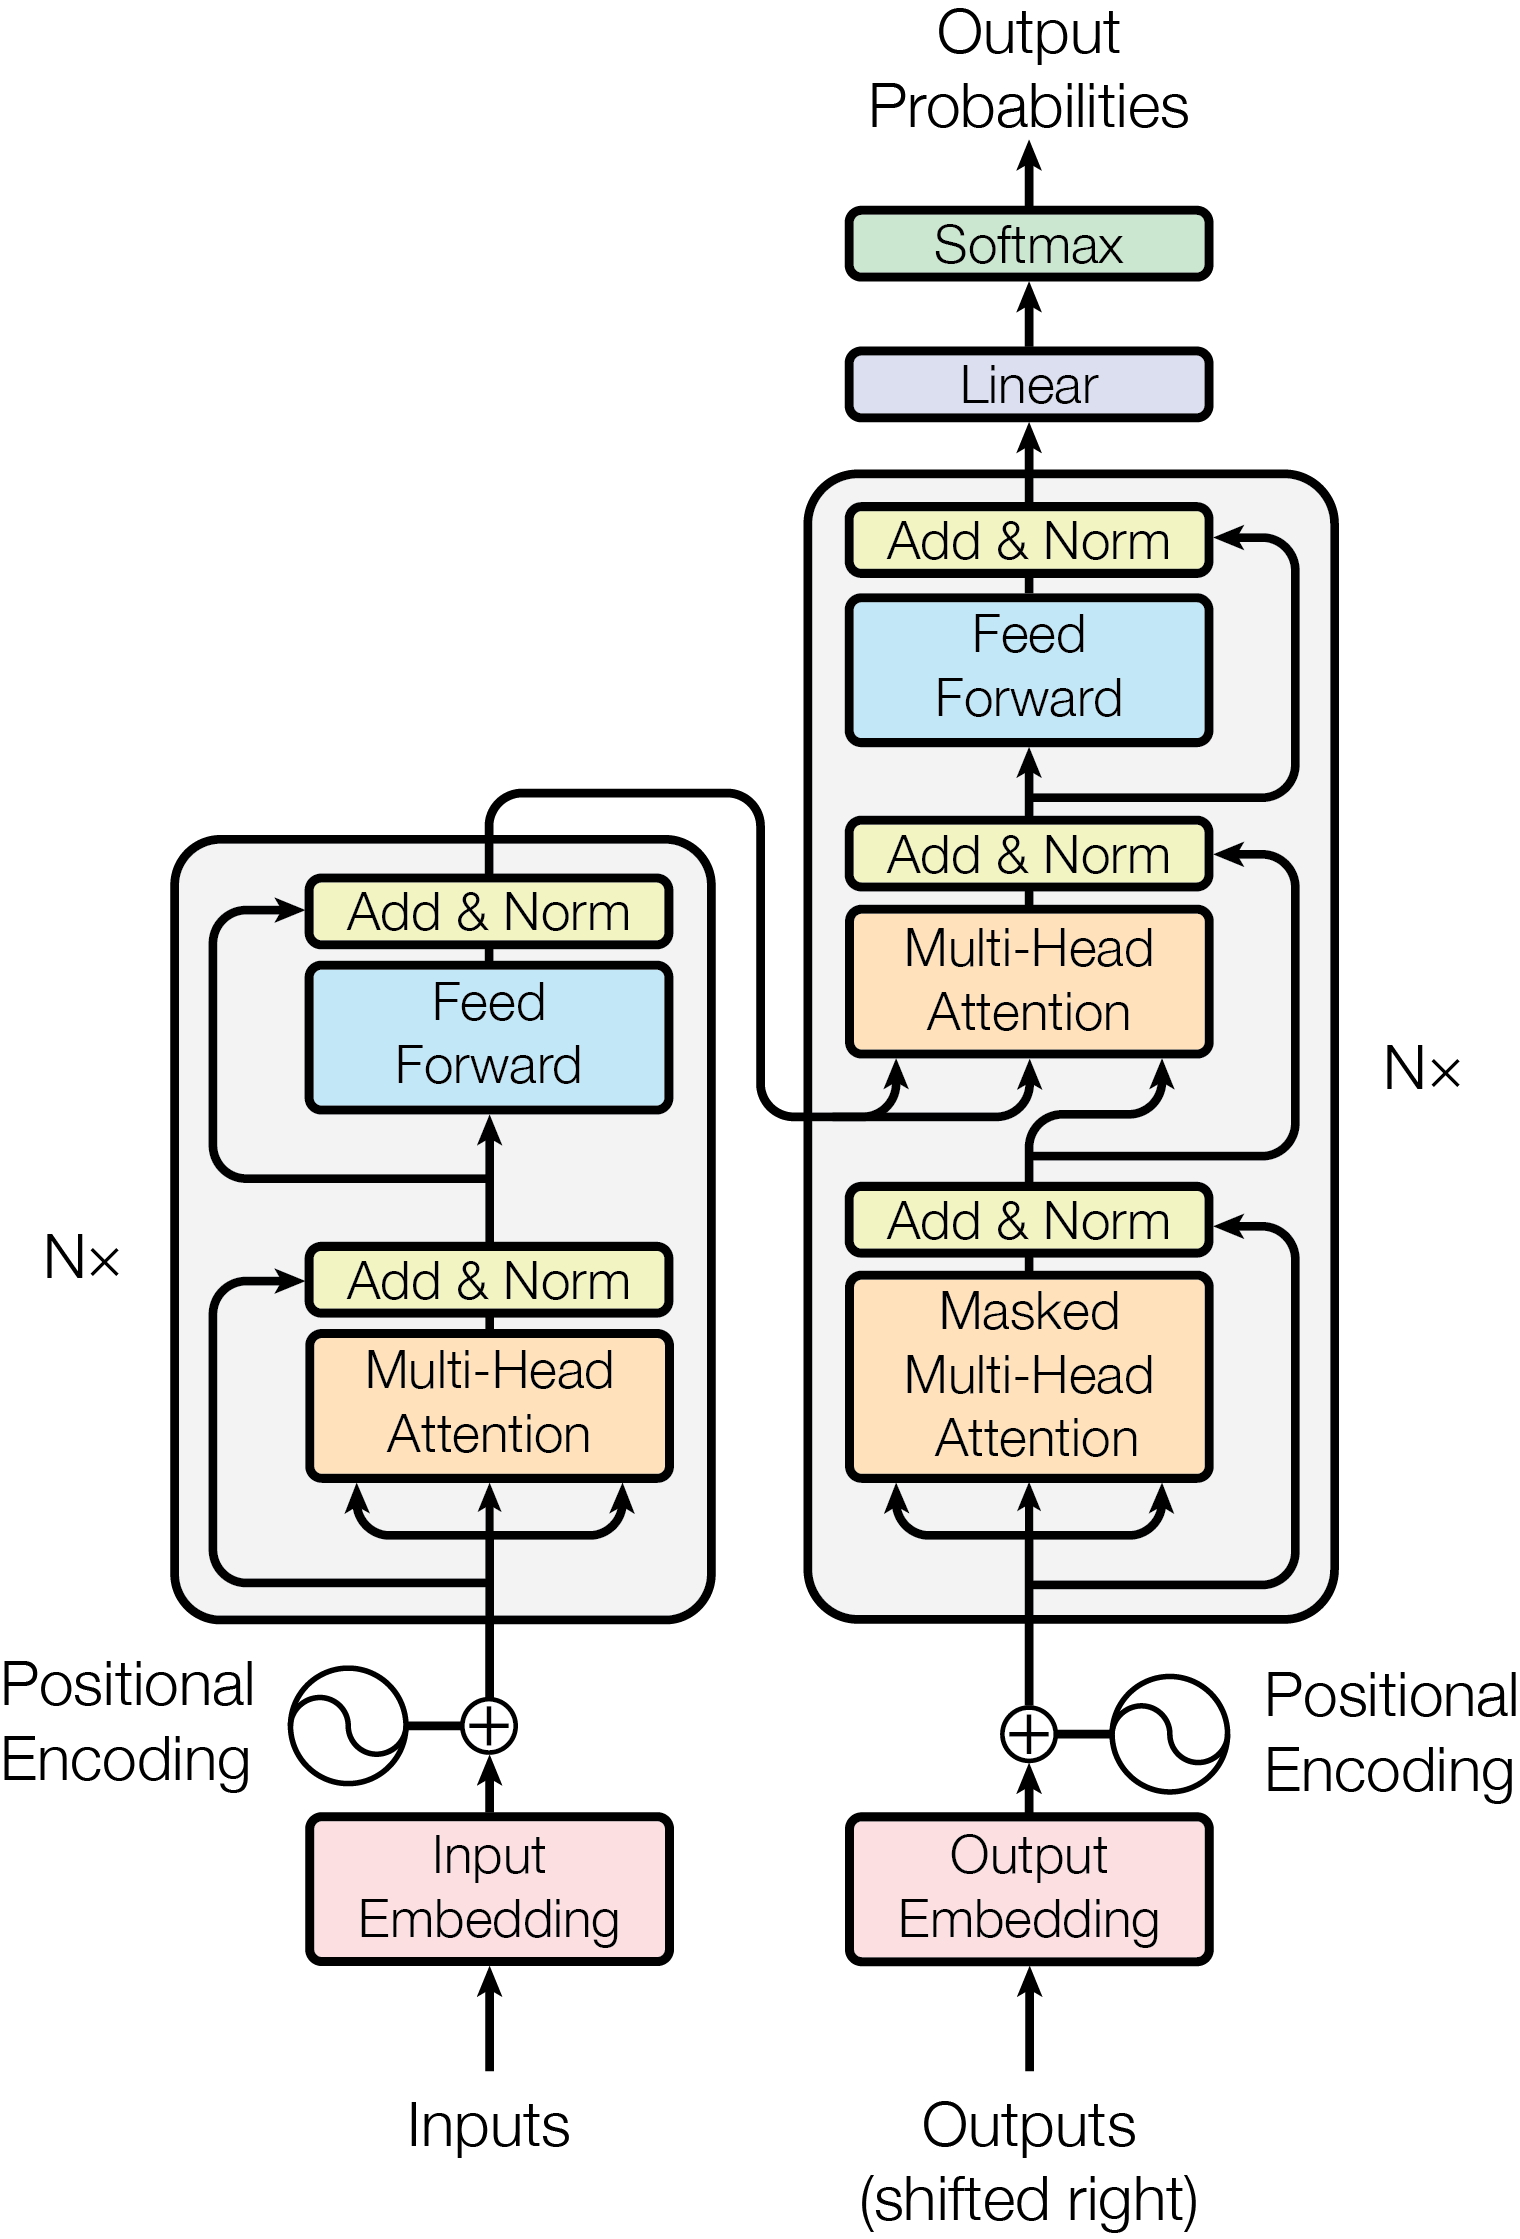
\includegraphics[width=0.60\textwidth]{Figures/ModalNet-21}
  \caption{The Transformer --- model architecture.}
  \label{fig:architecture}
\end{figure}

\subsection{Encoder and Decoder Stacks}
\textbf{Encoder:} The encoder is composed of a stack of $N=6$ identical layers.
Each layer has two sublayers. The first is a multi-head self-attention mechanism,
and the second is a simple, position-wise fully connected feed-forward network. We
employ a residual connection around each of the two sublayers, followed by layer
normalization~\citep{ba2016layer}. That is, the output of each sublayer is
$\mathrm{LayerNorm}(x + \mathrm{Sublayer}(x))$. To facilitate these residual
connections, all sublayers in the model, as well as the embedding layers, produce
outputs of dimension $\dmodel = 512$.

\textbf{Decoder:} The decoder is also composed of a stack of $N=6$ identical
layers. In addition to the two sublayers in each encoder layer, the decoder inserts
a third sublayer, which performs multi-head attention over the output of the
encoder stack. We modify the self-attention sublayer in the decoder stack (masking)
to prevent positions from attending to subsequent positions. This masking ensures
that the predictions for position $i$ can depend only on the known outputs at
positions less than $i$.

\subsection{Attention}
An attention function can be described as mapping a query and a set of key-value
pairs to an output, where the query, keys, values, and output are all vectors. The
output is computed as a weighted sum of the values, where the weight assigned to
each value is computed by a compatibility function of the query with the
corresponding key.

% ---- FIGURE 2: Scaled Dot-Product & Multi-Head Attention -------------------
\begin{figure}[t]
\begin{minipage}[t]{0.5\textwidth}
  \centering
  Scaled Dot-Product Attention \\[0.4cm]
  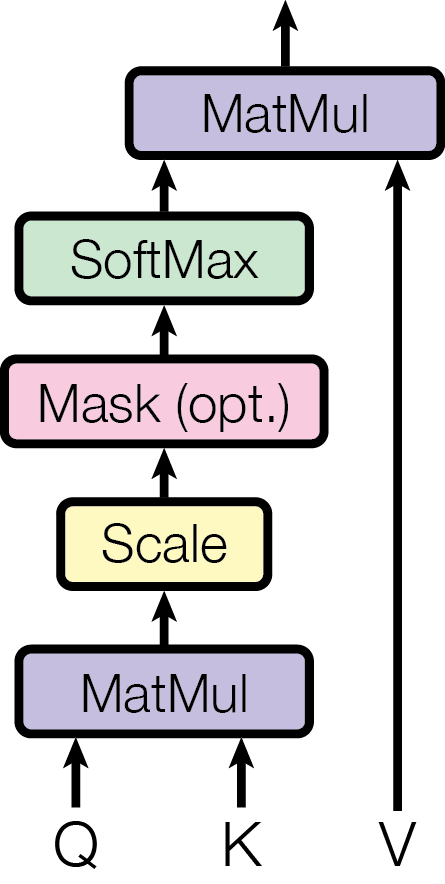
\includegraphics[height=5.2cm]{Figures/ModalNet-19}
\end{minipage}%
\begin{minipage}[t]{0.5\textwidth}
  \centering
  Multi-Head Attention \\[0.1cm]
  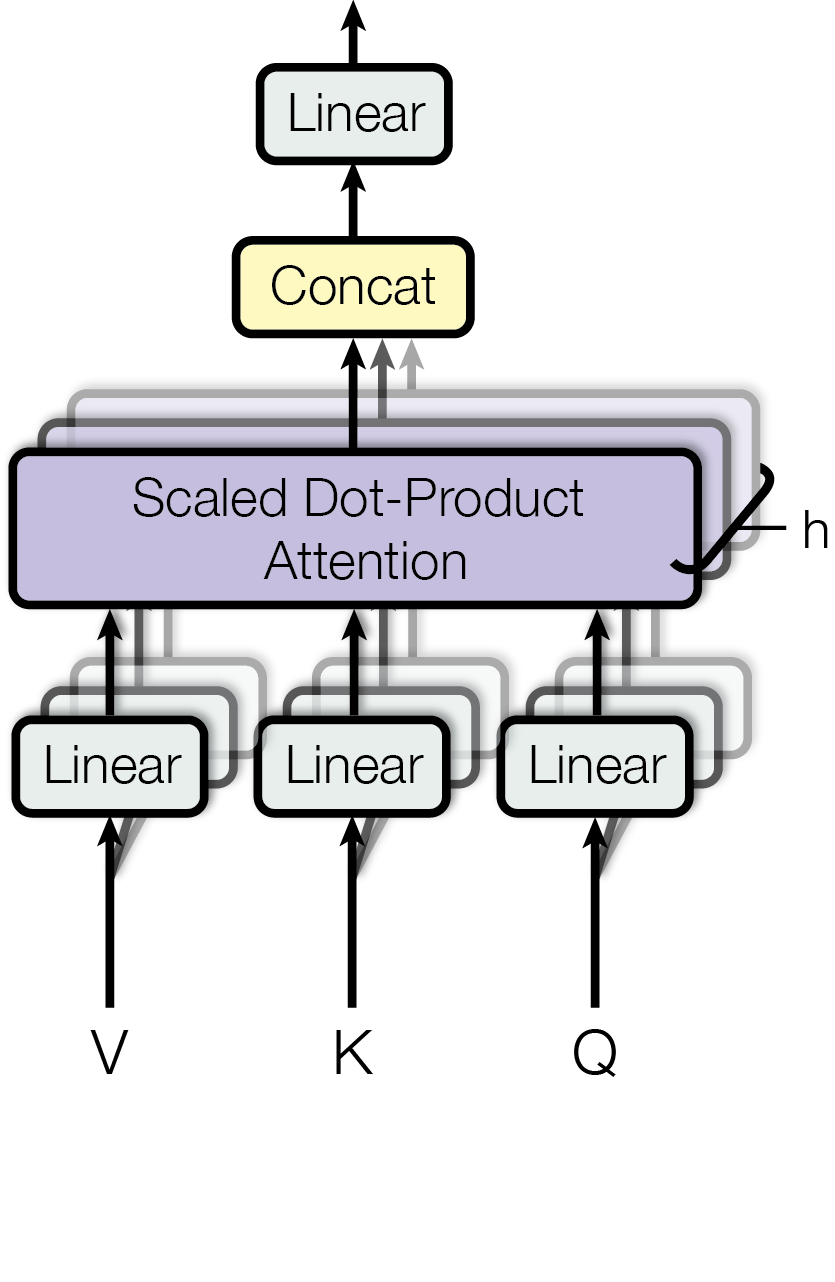
\includegraphics[height=5.2cm]{Figures/ModalNet-20}
\end{minipage}
  \caption{(left) Scaled Dot-Product Attention. (right) Multi-Head Attention
  consists of several attention layers running in parallel.}
  \label{fig:attention}
\end{figure}

\subsubsection{Scaled Dot-Product Attention}
We call our particular attention ``Scaled Dot-Product Attention''
(Figure~\ref{fig:attention}, left). The input consists of queries and keys of
dimension $d_k$, and values of dimension $d_v$. We compute the dot products of the
query with all keys, divide each by $\sqrt{d_k}$, and apply a softmax function to
obtain the weights on the values. In practice, we compute the attention function on
a set of queries simultaneously, packed together into a matrix $Q$. The keys and
values are also packed together into matrices $K$ and $V$. We compute the matrix of
outputs as:
\begin{equation}
  \Attention(Q,K,V) = \softmax\!\left(\frac{QK^{\top}}{\sqrt{d_k}}\right)V .
  \label{eq:attention}
\end{equation}

\subsubsection{Multi-Head Attention}
Instead of performing a single attention function with $\dmodel$-dimensional keys,
values and queries, we found it beneficial to linearly project the queries, keys
and values $h$ times with different, learned linear projections to $d_k$, $d_k$
and $d_v$ dimensions, respectively (Figure~\ref{fig:attention}, right). Multi-head
attention allows the model to jointly attend to information from different
representation subspaces at different positions:
\begin{align}
  \MultiHead(Q,K,V) &= \Concat(\head_1,\dots,\head_h)\,W^{O}, \\
  \text{where}\quad \head_i &= \Attention\!\left(QW_i^{Q}, KW_i^{K}, VW_i^{V}\right). \nonumber
\end{align}
Where the projections are parameter matrices $W_i^{Q}\in\mathbb{R}^{\dmodel\times d_k}$,
$W_i^{K}\in\mathbb{R}^{\dmodel\times d_k}$, $W_i^{V}\in\mathbb{R}^{\dmodel\times d_v}$
and $W^{O}\in\mathbb{R}^{hd_v\times \dmodel}$. In this work we employ $h=8$ parallel
attention layers, or heads. For each of these we use $d_k=d_v=\dmodel/h=64$.

\subsubsection{Applications of Attention in our Model}
The Transformer uses multi-head attention in three different ways: in
``encoder-decoder attention'' layers, the queries come from the previous decoder
layer, and the memory keys and values come from the output of the encoder; the
encoder contains self-attention layers where all of the keys, values and queries
come from the same place; and self-attention layers in the decoder allow each
position to attend to all positions up to and including that position.

\subsection{Position-wise Feed-Forward Networks}
In addition to attention sublayers, each of the layers in our encoder and decoder
contains a fully connected feed-forward network, which is applied to each position
separately and identically. This consists of two linear transformations with a
ReLU activation in between:
\begin{equation}
  \FFN(x) = \max(0,\; xW_1 + b_1)\,W_2 + b_2 .
  \label{eq:ffn}
\end{equation}
While the linear transformations are the same across different positions, they use
different parameters from layer to layer. The dimensionality of input and output is
$\dmodel = 512$, and the inner layer has dimensionality $\dff = 2048$.

\subsection{Embeddings and Softmax}
Similarly to other sequence transduction models, we use learned embeddings to
convert the input tokens and output tokens to vectors of dimension $\dmodel$. We
also use the usual learned linear transformation and softmax function to convert
the decoder output to predicted next-token probabilities. In our model, we share
the same weight matrix between the two embedding layers and the pre-softmax linear
transformation~\citep{press2017using}.

\subsection{Positional Encoding}
Since our model contains no recurrence and no convolution, in order for the model to
make use of the order of the sequence, we must inject some information about the
relative or absolute position of the tokens in the sequence. To this end, we add
``positional encodings'' to the input embeddings at the bottoms of the encoder and
decoder stacks. We use sine and cosine functions of different frequencies:
\begin{align}
  \PE_{(pos,\,2i)}   &= \sin\!\left(pos / 10000^{2i/\dmodel}\right), \\
  \PE_{(pos,\,2i+1)} &= \cos\!\left(pos / 10000^{2i/\dmodel}\right),
\end{align}
where $pos$ is the position and $i$ is the dimension.

% =============================================================================
\section{Why Self-Attention}
\label{sec:why}
In this section we compare various aspects of self-attention layers to the
recurrent and convolutional layers commonly used for mapping one variable-length
sequence of symbol representations to another sequence of equal length. Motivating
our use of self-attention we consider three desiderata: the total computational
complexity per layer; the amount of computation that can be parallelized, measured
by the minimum number of sequential operations required; and the path length
between long-range dependencies in the network. Table~\ref{tab:complexity}
summarizes these quantities for the different layer types.

% ---- TABLE 1 ---------------------------------------------------------------
\begin{table}[t]
\centering
\caption{Maximum path lengths, per-layer complexity and minimum number of
sequential operations for different layer types. $n$ is the sequence length, $d$ the
representation dimension, $k$ the convolution kernel size, and $r$ the neighbourhood
size in restricted self-attention.}
\label{tab:complexity}
\begin{tabular}{@{}lccc@{}}
\toprule
Layer Type & Complexity per Layer & Sequential Operations & Maximum Path Length \\
\midrule
Self-Attention              & $O(n^2\cdot d)$         & $O(1)$ & $O(1)$ \\
Recurrent                   & $O(n\cdot d^2)$         & $O(n)$ & $O(n)$ \\
Convolutional               & $O(k\cdot n\cdot d^2)$  & $O(1)$ & $O(\log_k(n))$ \\
Self-Attention (restricted) & $O(r\cdot n\cdot d)$    & $O(1)$ & $O(n/r)$ \\
\bottomrule
\end{tabular}
\end{table}

As noted in Table~\ref{tab:complexity}, a self-attention layer connects all
positions with a constant number of sequentially executed operations, whereas a
recurrent layer requires $O(n)$ sequential operations. In terms of computational
complexity, self-attention layers are faster than recurrent layers when the
sequence length $n$ is smaller than the representation dimensionality $d$, which is
most often the case with sentence representations used by state-of-the-art models.

% =============================================================================
\section{Training}
This section describes the training regime for our models.

\subsection{Training Data and Batching}
We trained on the standard WMT 2014 English-German dataset consisting of about 4.5
million sentence pairs. Sentences were encoded using byte-pair encoding, which has a
shared source-target vocabulary of about 37000 tokens. For English-French, we used
the significantly larger WMT 2014 English-French dataset consisting of 36M sentences.

\subsection{Hardware and Schedule}
We trained our models on one machine with eight NVIDIA P100 GPUs. For our base
models, each training step took about 0.4 seconds. We trained the base models for a
total of 100{,}000 steps or 12 hours. For our big models, step time was 1.0 seconds;
the big models were trained for 300{,}000 steps (3.5 days).

\subsection{Optimizer}
We used the Adam optimizer~\citep{kingma2015adam} with $\beta_1=0.9$,
$\beta_2=0.98$ and $\epsilon=10^{-9}$. We varied the learning rate over the course
of training, increasing it linearly for the first \emph{warmup} steps and decreasing
it thereafter proportionally to the inverse square root of the step number.

\subsection{Regularization}
We employ three types of regularization during training: residual dropout applied to
the output of each sublayer~\citep{srivastava2014dropout}; dropout applied to the
sums of the embeddings and the positional encodings; and label
smoothing~\citep{szegedy2016rethinking} of value $\epsilon_{ls}=0.1$.

% =============================================================================
\section{Results}
\subsection{Machine Translation}
On the WMT 2014 English-to-German translation task, the big Transformer model
outperforms the best previously reported models (including ensembles) by more than
2.0 BLEU, establishing a new state-of-the-art BLEU score of 28.4. On the WMT 2014
English-to-French translation task, our big model achieves a BLEU score of 41.8,
outperforming all of the previously published single models, at less than $1/4$ the
training cost of the previous state-of-the-art model. Table~\ref{tab:results}
summarizes our results and compares translation quality and training costs to other
model architectures from the literature.

% ---- TABLE 2 ---------------------------------------------------------------
\begin{table}[t]
\centering
\caption{The Transformer achieves better BLEU scores than previous
state-of-the-art models on the English-to-German and English-to-French
newstest2014 tests at a fraction of the training cost.}
\label{tab:results}
\begin{tabular}{@{}lcccc@{}}
\toprule
\multirow{2}{*}{Model} & \multicolumn{2}{c}{BLEU} & \multicolumn{2}{c}{Training Cost (FLOPs)} \\
\cmidrule(lr){2-3}\cmidrule(l){4-5}
 & EN-DE & EN-FR & EN-DE & EN-FR \\
\midrule
ByteNet \citep{kalchbrenner2016neural}            & 23.75 &       &                   &  \\
Deep-Att + PosUnk \citep{zhou2016deep}            &       & 39.2  &                   & $1.0\cdot10^{20}$ \\
GNMT + RL \citep{wu2016google}                    & 24.6  & 39.92 & $2.3\cdot10^{19}$ & $1.4\cdot10^{20}$ \\
ConvS2S \citep{gehring2017convolutional}          & 25.16 & 40.46 & $9.6\cdot10^{18}$ & $1.5\cdot10^{20}$ \\
MoE \citep{shazeer2017outrageously}               & 26.03 & 40.56 & $2.0\cdot10^{19}$ & $1.2\cdot10^{20}$ \\
\midrule
GNMT + RL Ensemble \citep{wu2016google}           & 26.30 & 41.16 & $1.8\cdot10^{20}$ & $1.1\cdot10^{21}$ \\
ConvS2S Ensemble \citep{gehring2017convolutional} & 26.36 & 41.29 & $7.7\cdot10^{19}$ & $1.2\cdot10^{21}$ \\
\midrule
Transformer (base model) & 27.3 & 38.1 & \multicolumn{2}{c}{$3.3\cdot10^{18}$} \\
Transformer (big)        & \textbf{28.4} & \textbf{41.8} & \multicolumn{2}{c}{$2.3\cdot10^{19}$} \\
\bottomrule
\end{tabular}
\end{table}

\subsection{Model Variations}
To evaluate the importance of different components of the Transformer, we varied our
base model in different ways, measuring the change in performance on English-to-German
translation on the development set, newstest2013. We present these results in
Table~\ref{tab:variations}.

% ---- TABLE 3 (wide — wrapped in \resizebox to guarantee fit) ---------------
\begin{table}[t]
\centering
\caption{Variations on the Transformer architecture. Unlisted values are identical
to those of the base model. All metrics are on the English-to-German translation
development set, newstest2013.}
\label{tab:variations}
\resizebox{\textwidth}{!}{%
\setlength{\tabcolsep}{4pt}
\begin{tabular}{@{}cccccccccccccc@{}}
\toprule
 & $N$ & $\dmodel$ & $\dff$ & $h$ & $d_k$ & $d_v$ & $P_{drop}$ & $\epsilon_{ls}$ &
 train steps & PPL (dev) & BLEU (dev) & params ($\times10^6$) \\
\midrule
base & 6 & 512 & 2048 & 8 & 64 & 64 & 0.1 & 0.1 & 100K & 4.92 & 25.8 & 65 \\
\midrule
\multirow{4}{*}{(A)}
     &   &     &      & 1  & 512 & 512 &     &     &      & 5.29 & 24.9 &     \\
     &   &     &      & 4  & 128 & 128 &     &     &      & 5.00 & 25.5 &     \\
     &   &     &      & 16 & 32  & 32  &     &     &      & 4.91 & 25.8 &     \\
     &   &     &      & 32 & 16  & 16  &     &     &      & 5.01 & 25.4 &     \\
\midrule
\multirow{2}{*}{(B)}
     &   &     &      &    & 16  &     &     &     &      & 5.16 & 25.1 & 58  \\
     &   &     &      &    & 32  &     &     &     &      & 5.01 & 25.4 & 60  \\
\midrule
\multirow{7}{*}{(C)}
     & 2 &     &      &    &     &     &     &     &      & 6.11 & 23.7 & 36  \\
     & 4 &     &      &    &     &     &     &     &      & 5.19 & 25.3 & 50  \\
     & 8 &     &      &    &     &     &     &     &      & 4.88 & 25.5 & 80  \\
     &   & 256 &      &    & 32  & 32  &     &     &      & 5.75 & 24.5 & 28  \\
     &   & 1024&      &    & 128 & 128 &     &     &      & 4.66 & 26.0 & 168 \\
     &   &     & 1024 &    &     &     &     &     &      & 5.12 & 25.4 & 53  \\
     &   &     & 4096 &    &     &     &     &     &      & 4.75 & 26.2 & 90  \\
\midrule
\multirow{4}{*}{(D)}
     &   &     &      &    &     &     & 0.0 &     &      & 5.77 & 24.6 &     \\
     &   &     &      &    &     &     & 0.2 &     &      & 4.95 & 25.5 &     \\
     &   &     &      &    &     &     &     & 0.0 &      & 4.67 & 25.3 &     \\
     &   &     &      &    &     &     &     & 0.2 &      & 5.47 & 25.7 &     \\
\midrule
(E)  & \multicolumn{9}{c}{positional embedding instead of sinusoids} & 4.92 & 25.7 & \\
\midrule
big  & 6 & 1024 & 4096 & 16 & 64 & 64 & 0.3 & 0.1 & 300K & 4.33 & 26.4 & 213 \\
\bottomrule
\end{tabular}%
}
\end{table}

\subsection{English Constituency Parsing}
To evaluate whether the Transformer can generalize to other tasks we performed
experiments on English constituency parsing. Despite the lack of task-specific
tuning, our model performs surprisingly well, yielding better results than all
previously reported models with the exception of the Recurrent Neural Network
Grammar. In contrast to RNN sequence-to-sequence models, the Transformer
outperforms previously reported approaches even when training only on the WSJ
training set of 40K sentences.

% =============================================================================
\section{Conclusion}
In this work, we presented the Transformer, the first sequence transduction model
based entirely on attention, replacing the recurrent layers most commonly used in
encoder-decoder architectures with multi-head self-attention. For translation tasks,
the Transformer can be trained significantly faster than architectures based on
recurrent or convolutional layers. On both WMT 2014 English-to-German and WMT 2014
English-to-French translation tasks we achieve a new state of the art. We are
excited about the future of attention-based models and plan to apply them to other
tasks and other modalities.

\subsubsection*{Acknowledgments}
We are grateful to Nal Kalchbrenner and Stephan Gouws for their fruitful comments,
corrections and inspiration. This document is a typesetting demonstration for the
\texttt{kirklin} LaTeX skill and is not the original publication.

% ---- References ------------------------------------------------------------
\bibliographystyle{unsrtnat}
\bibliography{references}

% =============================================================================
%  Appendix — the paper's real attention-weight visualizations (vis/*.pdf)
% =============================================================================
\clearpage
\section*{Attention Visualizations}
\begin{figure}[h]
  \centering
  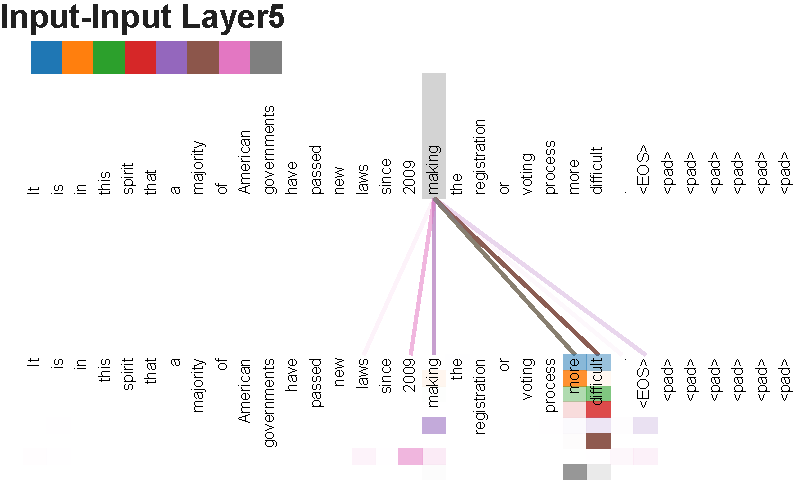
\includegraphics[width=\textwidth, trim=0 0 0 36, clip]{vis/making_more_difficult5_new.pdf}
  \caption{An example of the attention mechanism following long-distance
  dependencies in the encoder self-attention in layer 5 of 6. Many of the attention
  heads attend to a distant dependency of the verb `making', completing the phrase
  `making\ldots more difficult'. Attentions here shown only for the word `making'.
  Different colors represent different heads. Best viewed in color.}
\end{figure}

\begin{figure}[h]
  \centering
  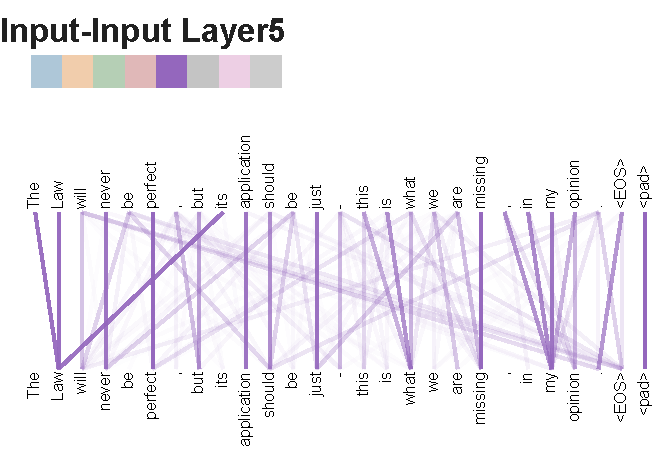
\includegraphics[width=\textwidth, trim=0 0 0 45, clip]{vis/anaphora_resolution_new.pdf}\\[1.5ex]
  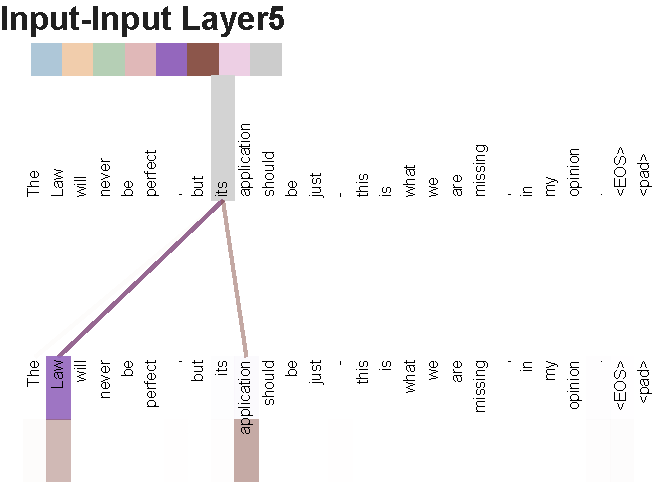
\includegraphics[width=\textwidth, trim=0 0 0 37, clip]{vis/anaphora_resolution2_new.pdf}
  \caption{Two attention heads, also in layer 5 of 6, apparently involved in
  anaphora resolution. Top: Full attentions for head 5. Bottom: Isolated attentions
  from just the word `its' for attention heads 5 and 6. Note that the attentions are
  very sharp for this word.}
\end{figure}

\begin{figure}[h]
  \centering
  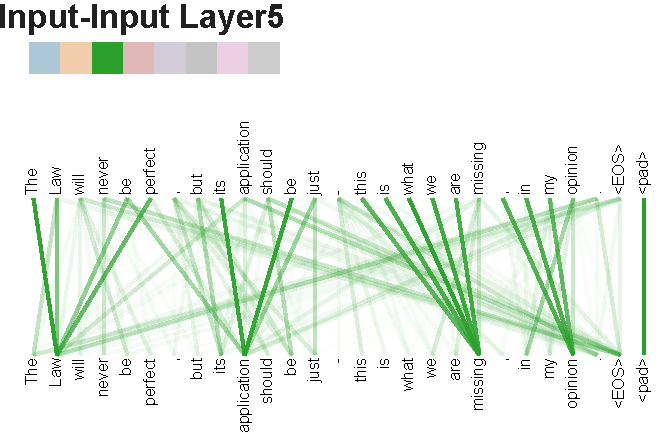
\includegraphics[width=\textwidth, trim=0 0 0 36, clip]{vis/attending_to_head_new.pdf}\\[1.5ex]
  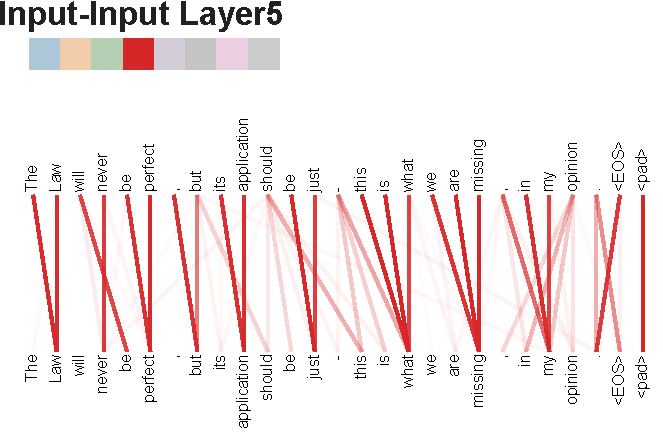
\includegraphics[width=\textwidth, trim=0 0 0 36, clip]{vis/attending_to_head2_new.pdf}
  \caption{Many of the attention heads exhibit behaviour that seems related to the
  structure of the sentence. We give two such examples above, from two different
  heads from the encoder self-attention at layer 5 of 6. The heads clearly learned
  to perform different tasks.}
\end{figure}

\end{document}
